\documentclass[11pt]{article}
\usepackage[margin=1in]{geometry}
\usepackage{amsmath,amssymb,graphicx,booktabs,xcolor,fancyvrb}
\usepackage[colorlinks=true,linkcolor=blue]{hyperref}

\makeatletter
\def\ps@hw{%
  \def\@oddhead{\itshape\small CS 334 HW1 --- Written Submission\hfill Nathaniel Schrader}%
  \def\@oddfoot{\hfil\small\thepage\hfil}%
  \let\@evenhead\@oddhead \let\@evenfoot\@oddfoot}
\makeatother
\pagestyle{hw}

\fvset{fontsize=\footnotesize,frame=single,numbers=left,numbersep=4pt,xleftmargin=6pt}
\newcommand{\R}{\mathbb{R}}

\begin{document}
\thispagestyle{hw}

\begin{center}
{\Large\bfseries CS 334 --- Homework 1 Submission}\\[4pt]
{\large Nathaniel Schrader \quad|\quad CS 334 Section 2 \quad|\quad Fall 2026}\\[10pt]
\fbox{\parbox{0.92\textwidth}{\small\centering
\textbf{Honor Code Statement:}\\
THIS HOMEWORK IS MY OWN WORK, WRITTEN WITHOUT COPYING FROM OTHER STUDENTS
OR DIRECTLY FROM LARGE LANGUAGE MODELS SUCH AS CHATGPT.\\
Any collaboration or external resources have been properly acknowledged.\\[4pt]
\textit{Nathaniel Schrader}}}
\end{center}
\vspace{6pt}
\hrule
\vspace{10pt}

\section*{Q1 --- Vectors \& Planes Review}

\paragraph{(a)} Given two 3-dimensional vectors $\vec{x}^{(1)}=[a_1,a_2,a_3]^T$ and $\vec{x}^{(2)}=[a_1,a_3,-a_2]^T$ in $\R^3$:
\[ \vec{x}^{(1)}\cdot\vec{x}^{(2)} = a_1^2 + a_2a_3 + a_3(-a_2) = a_1^2 \]
Both vectors have norm $\|\vec{x}^{(1)}\|=\|\vec{x}^{(2)}\|=\sqrt{a_1^2+a_2^2+a_3^2}$, so the angle $\theta$ between them satisfies:
\[ \cos\theta = \frac{\vec{x}^{(1)}\cdot\vec{x}^{(2)}}{\|\vec{x}^{(1)}\|\|\vec{x}^{(2)}\|} = \frac{a_1^2}{a_1^2+a_2^2+a_3^2}, \qquad \theta = \arccos\!\left(\frac{a_1^2}{\|\vec{x}^{(1)}\|^2}\right) \]
The vectors are orthogonal if and only if $\vec{x}^{(1)}\cdot\vec{x}^{(2)} = 0 \iff a_1^2=0 \iff \boxed{a_1=0}$ (assuming non-zero vectors, i.e., $a_2,a_3$ not both zero).

\paragraph{(b)} Any non-zero scalar multiple $c\vec{\theta}$ for any $c\in\R\setminus\{0\}$ (such as $-\vec{\theta}$). Multiplying the equation $\vec{\theta}\cdot\vec{x}=0$ by $c$ yields $c(\vec{\theta}\cdot\vec{x})=0$, which defines the same plane.
There are infinitely many such alternative normal vectors, forming the line $\mathrm{span}(\vec{\theta})$ excluding the origin.

\paragraph{(c)} The signed distance from $\vec{x}$ to $\vec{\theta}\cdot\vec{x}+b=0$ is:
\[ \text{distance} = \frac{\vec{\theta}\cdot\vec{x}+b}{\|\vec{\theta}\|} \]
For $\vec\theta=[1,-2]^T$ and $\vec a=[-1,1]^T$, we have $\|\vec\theta\|=\sqrt{1^2+(-2)^2}=\sqrt{5}$ and $\vec\theta\cdot\vec a = -3$.
\begin{itemize}\itemsep2pt
\item[(i)] Plane $p_1$ ($b=0$): \quad $\dfrac{-3}{\sqrt5} = \boxed{-\tfrac{3}{\sqrt5}\approx-1.3416}$
\item[(ii)] Plane $p_2$ ($b=5$): \quad $\dfrac{-3+5}{\sqrt5} = \boxed{\tfrac{2}{\sqrt5}\approx+0.8944}$
\end{itemize}
The sign flips because $\vec a$ lies on the side opposite to $\vec\theta$ for plane $p_1$, but on the same side for plane $p_2$.

\paragraph{(d)} The original point cannot be uniquely recovered. Orthogonal projection onto a hyperplane removes the displacement component along the normal vector $\vec{\theta}$, so infinitely many points map to the same projected point $\vec{x}^{(0)}$.
All points projecting to $\vec{x}^{(0)}$ lie on the normal line:
\[ \left\{\, \vec{x}^{(0)} + t\,\vec{\theta} \;:\; t\in\R \,\right\} \qquad\text{or}\qquad \left\{\, \vec{x}^{(0)} + t\,\frac{\vec{\theta}}{\|\vec{\theta}\|} \;:\; t\in\R \,\right\} \]

\section*{Q2 --- Linear Algebra Review}

\paragraph{(a)} For an $m$-dimensional column vector $\vec{v}=[v_1, v_2, \dots, v_m]^T$:
\begin{itemize}\itemsep2pt
\item[i.] $\displaystyle\sum_{i=1}^m v_i v_i = \vec{v}^T\vec{v}$
\item[ii.] $\displaystyle\sum_{i=1}^m v_i v_i = \|\vec{v}\|^2$
\item[iii.] The matrix $C$ with $c_{ij} = v_i v_j$ is the outer product $C = \vec{v}\,\vec{v}^T$.
\end{itemize}

\paragraph{(b)} The sum of squared errors in matrix-vector form is:
\[ \sum_{i=1}^n\left(\vec{\theta}\cdot\vec{x}^{(i)}-y^{(i)}\right)^2 = \left\|X\vec{\theta}-\vec{y}\right\|^2 = \left(X\vec{\theta}-\vec{y}\right)^T\left(X\vec{\theta}-\vec{y}\right) \]

\paragraph{(c)} False. The correct transpose property is $(AB)^T=B^TA^T$.
Counterexample: Let $A=\begin{bmatrix}1&1\end{bmatrix}$ ($1\times2$) and $B=\begin{bmatrix}1\\2\end{bmatrix}$ ($2\times1$).
Then $AB=\begin{bmatrix}3\end{bmatrix}$ ($1\times1$), so $(AB)^T=\begin{bmatrix}3\end{bmatrix}$.
However, $A^TB^T = \begin{bmatrix}1\\1\end{bmatrix}\begin{bmatrix}1&2\end{bmatrix} = \begin{bmatrix}1&2\\1&2\end{bmatrix}$ ($2\times2$).
Because $(AB)^T$ is $1\times1$ while $A^TB^T$ is $2\times2$, $(AB)^T \neq A^TB^T$ in general.

\paragraph{(d)} Not possible. By rank properties of matrix multiplication:
\[ \mathrm{rank}(C)=\mathrm{rank}(AB)\le\min\{\mathrm{rank}(A),\mathrm{rank}(B)\}\le\min\{n,p\}=p \]
With $p < n$, we have $\mathrm{rank}(C) \le p < n$, so $C \in \R^{n\times n}$ is always rank-deficient.

\newpage
\section*{Q3(f) --- Vectorization Timing Comparison}

Below are the execution times for `sum\_squares\_for` vs `sum\_squares\_np` for sample sizes $n$ from $10$ to $10^7$:

\begin{center}\small
\begin{tabular}{rrrr}
\toprule
$n$ & \texttt{ssfor} (s) & \texttt{ssnp} (s) & Speedup ($\times$) \\
\midrule
10 & 0.000010 & 0.000009 & 1.1$\times$ \\
100 & 0.000015 & 0.000002 & 7.3$\times$ \\
1{,}000 & 0.000118 & 0.000002 & 56.6$\times$ \\
1{,}000 & 0.001269 & 0.000009 & 144.4$\times$ \\
100{,}000 & 0.011674 & 0.000081 & 144.9$\times$ \\
1{,}000{,}000 & 0.117380 & 0.000978 & 120.1$\times$ \\
10{,}000{,}000 & 1.128647 & 0.008340 & 135.3$\times$ \\
\bottomrule
\end{tabular}
\end{center}

\begin{center}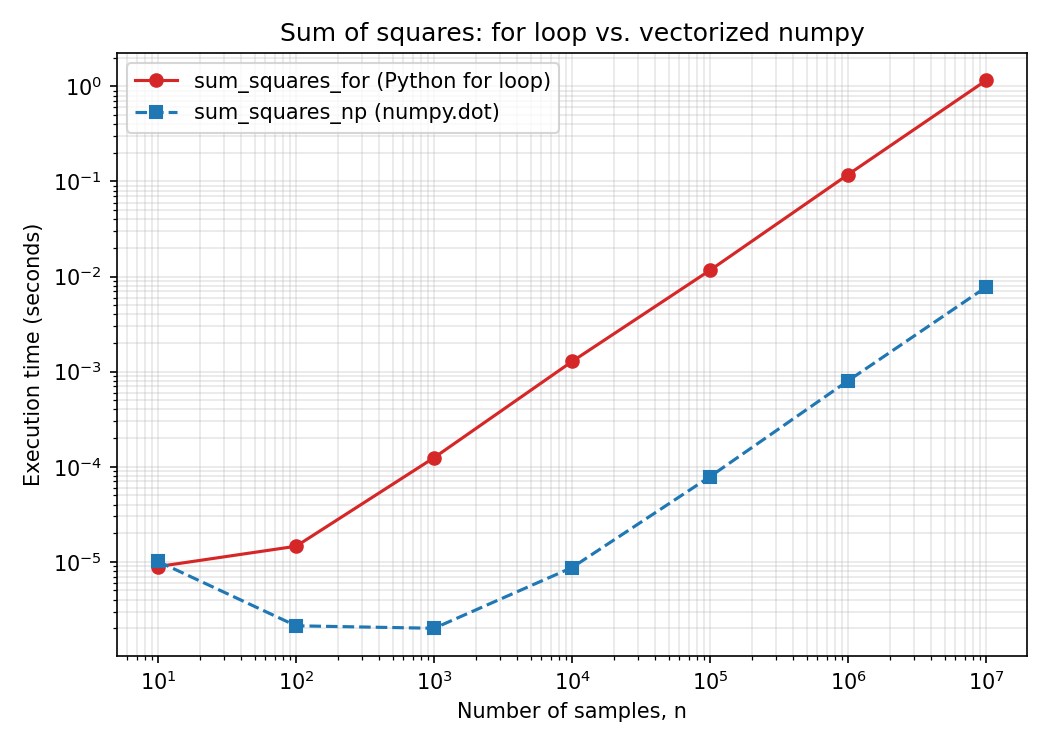
\includegraphics[width=0.75\textwidth]{figures/q3f_timing.png}\end{center}

\paragraph{Discussion.} Both implementations scale in $O(n)$ time, shown by parallel lines of slope $\approx 1$ on the log--log plot. NumPy's \texttt{np.dot} is roughly $120\times$--$145\times$ faster at large $n$ because its iteration runs in compiled C rather than through Python's bytecode loop. At $n=10$, function call overhead dominates the actual calculation, so execution times are nearly identical.

\paragraph{Code.}
\begin{Verbatim}
import timeit
import numpy as np
import pandas as pd
import matplotlib.pyplot as plt

def run_timing_sweep():
    sample_list = [10, 100, 1000, 10_000, 100_000, 1_000_000, 10_000_000]
    df = timess_to_df(time_ss(sample_list))
    
    fig, ax = plt.subplots(figsize=(7, 5))
    ax.loglog(df["n"], df["ssfor"], marker="o", color="tab:red", label="sum_squares_for")
    ax.loglog(df["n"], df["ssnp"], marker="s", color="tab:blue", label="sum_squares_np")
    ax.set_xlabel("Number of samples, n")
    ax.set_ylabel("Execution time (seconds)")
    ax.set_title("Sum of squares: for loop vs. vectorized numpy")
    ax.grid(True, which="both", alpha=0.3)
    ax.legend()
    fig.tight_layout()
    fig.savefig("figures/q3f_timing.png", dpi=150)
\end{Verbatim}

\newpage
\section*{Q5(a) --- Species Distribution Before and After Dropping NaNs}

\begin{center}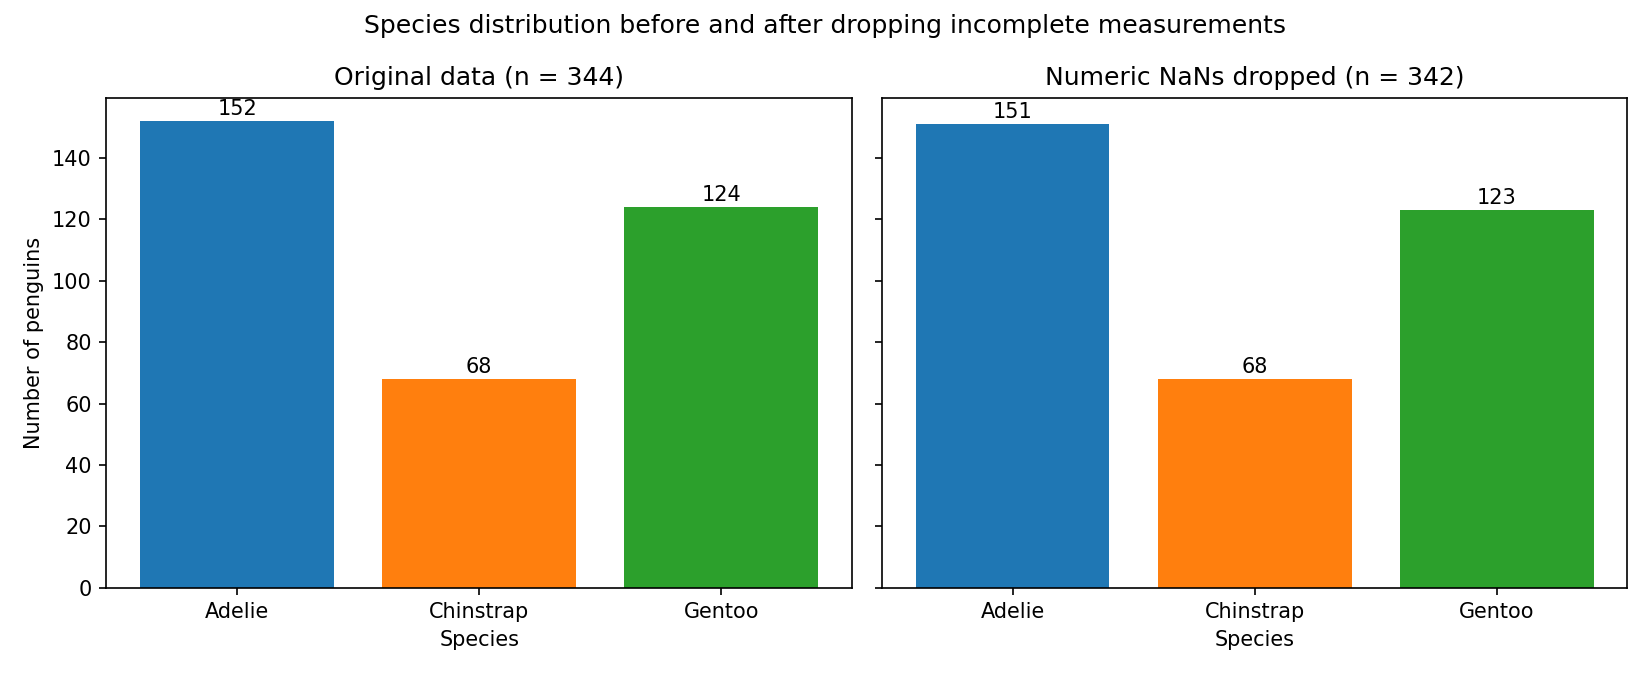
\includegraphics[width=0.95\textwidth]{figures/q5a_species_histograms.png}\end{center}

\begin{center}\small
\begin{tabular}{lrrrr}
\toprule
& Adelie & Chinstrap & Gentoo & Total \\
\midrule
Original Count & 152 & 68 & 124 & 344 \\
NaNs Dropped Count & 151 & 68 & 123 & 342 \\
\midrule
Original Proportion (\%) & 44.19\% & 19.77\% & 36.05\% & 100.0\% \\
NaNs Dropped Proportion (\%) & 44.15\% & 19.88\% & 35.96\% & 100.0\% \\
\bottomrule
\end{tabular}
\end{center}

\paragraph{Does dropping incomplete measurements change the species distribution?}
No. Dropping rows with missing numeric values removes only 2 out of 344 entries (one Adelie and one Gentoo). The relative proportions change by less than 0.15 percentage points across all species, keeping the overall distribution and species ordering ($\text{Adelie} > \text{Gentoo} > \text{Chinstrap}$) intact.

\newpage
\section*{Q5(b) --- Numeric Features by Species}

\begin{center}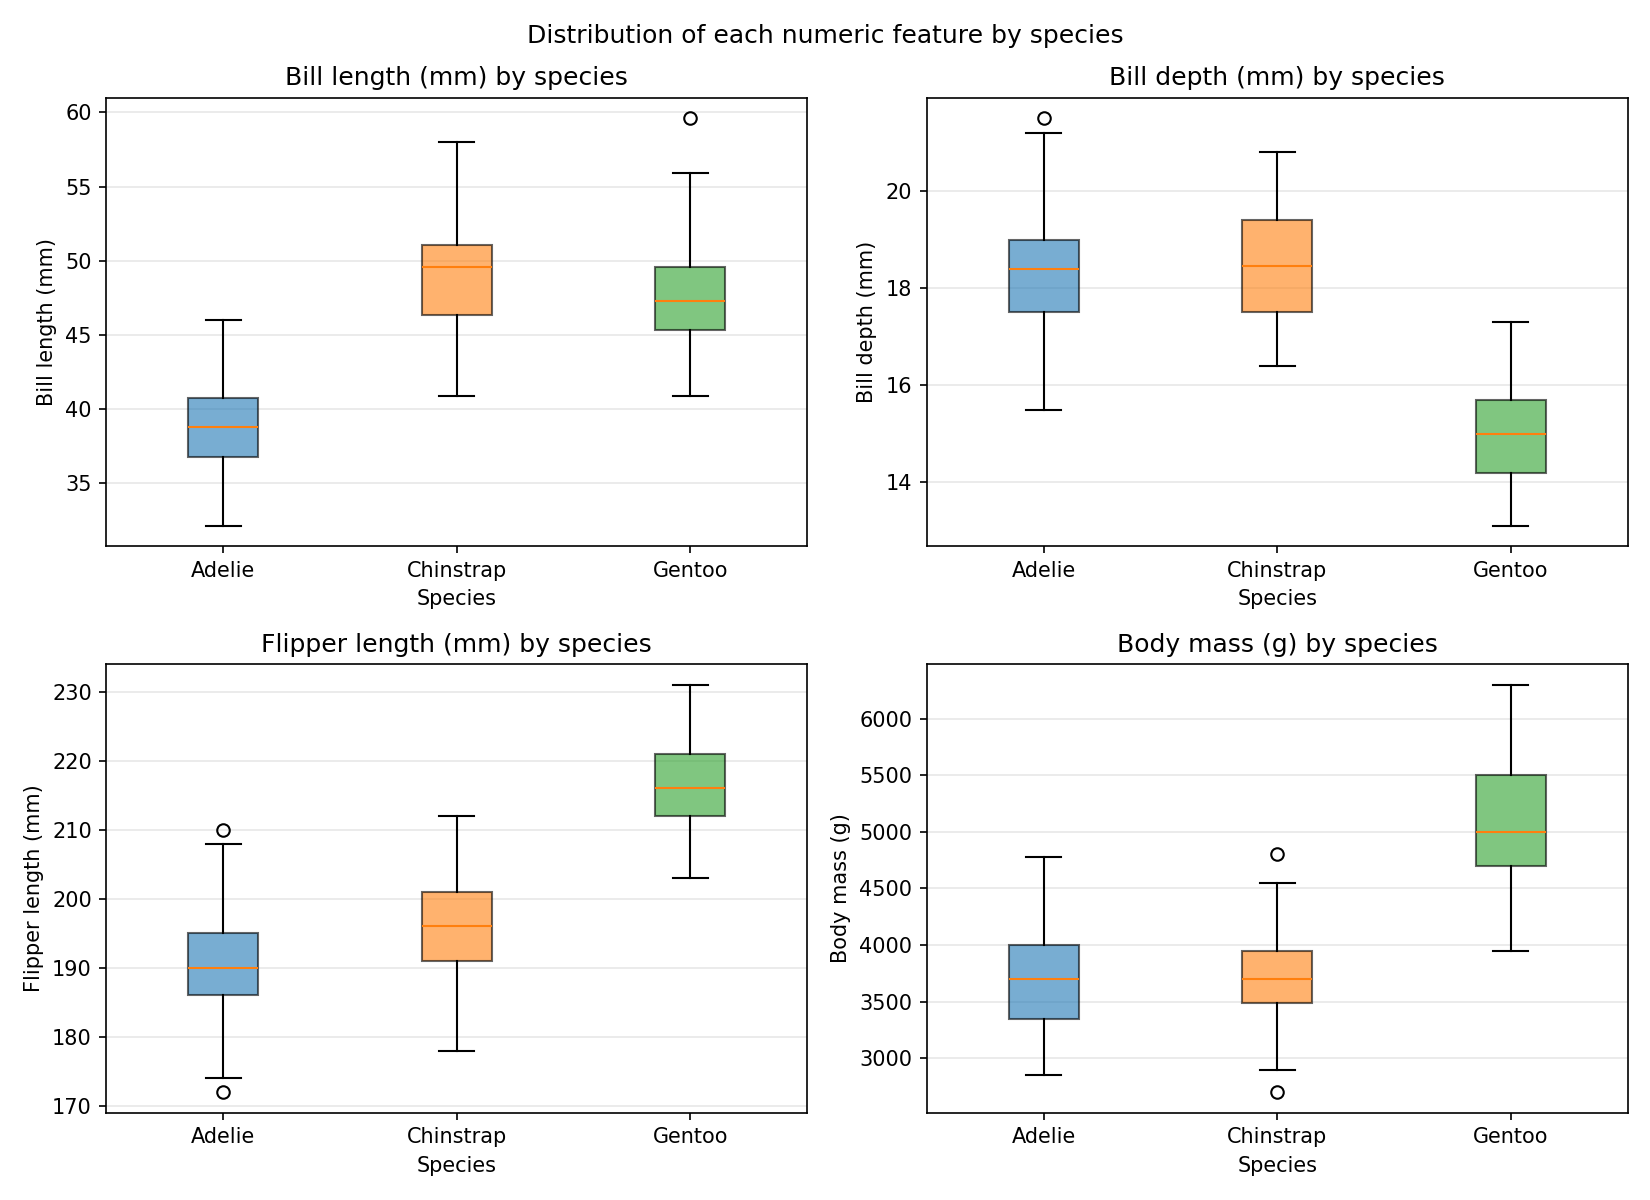
\includegraphics[width=0.95\textwidth]{figures/q5b_boxplots.png}\end{center}

\begin{center}\small
\begin{tabular}{lccc}
\toprule
Median [Min, Max] & Adelie & Chinstrap & Gentoo \\
\midrule
Bill length (mm) & 38.8 [32.1, 46.0] & 49.5 [40.9, 58.0] & 47.3 [40.9, 59.6] \\
Bill depth (mm) & 18.4 [15.5, 21.5] & 18.4 [16.4, 20.8] & \textbf{15.0 [13.1, 17.3]} \\
Flipper length (mm) & 190 [172, 210] & 196 [178, 212] & \textbf{216 [203, 231]} \\
Body mass (g) & 3700 [2850, 4775] & 3700 [2700, 4800] & \textbf{5000 [3950, 6300]} \\
\bottomrule
\end{tabular}
\end{center}

\paragraph{Observations.} Gentoo penguins differ from the other two species across bill depth, flipper length, and body mass, with a median bill depth of 15.0 mm compared to 18.4 mm for Adelie and Chinstrap. Adelie and Chinstrap have matching medians for bill depth (18.4 mm) and body mass (3700 g), but separate on bill length (median 38.8 mm for Adelie vs 49.5 mm for Chinstrap).

\newpage
\section*{Q5(c) --- Pairwise Scatterplots \& Simpson's Paradox}

\begin{center}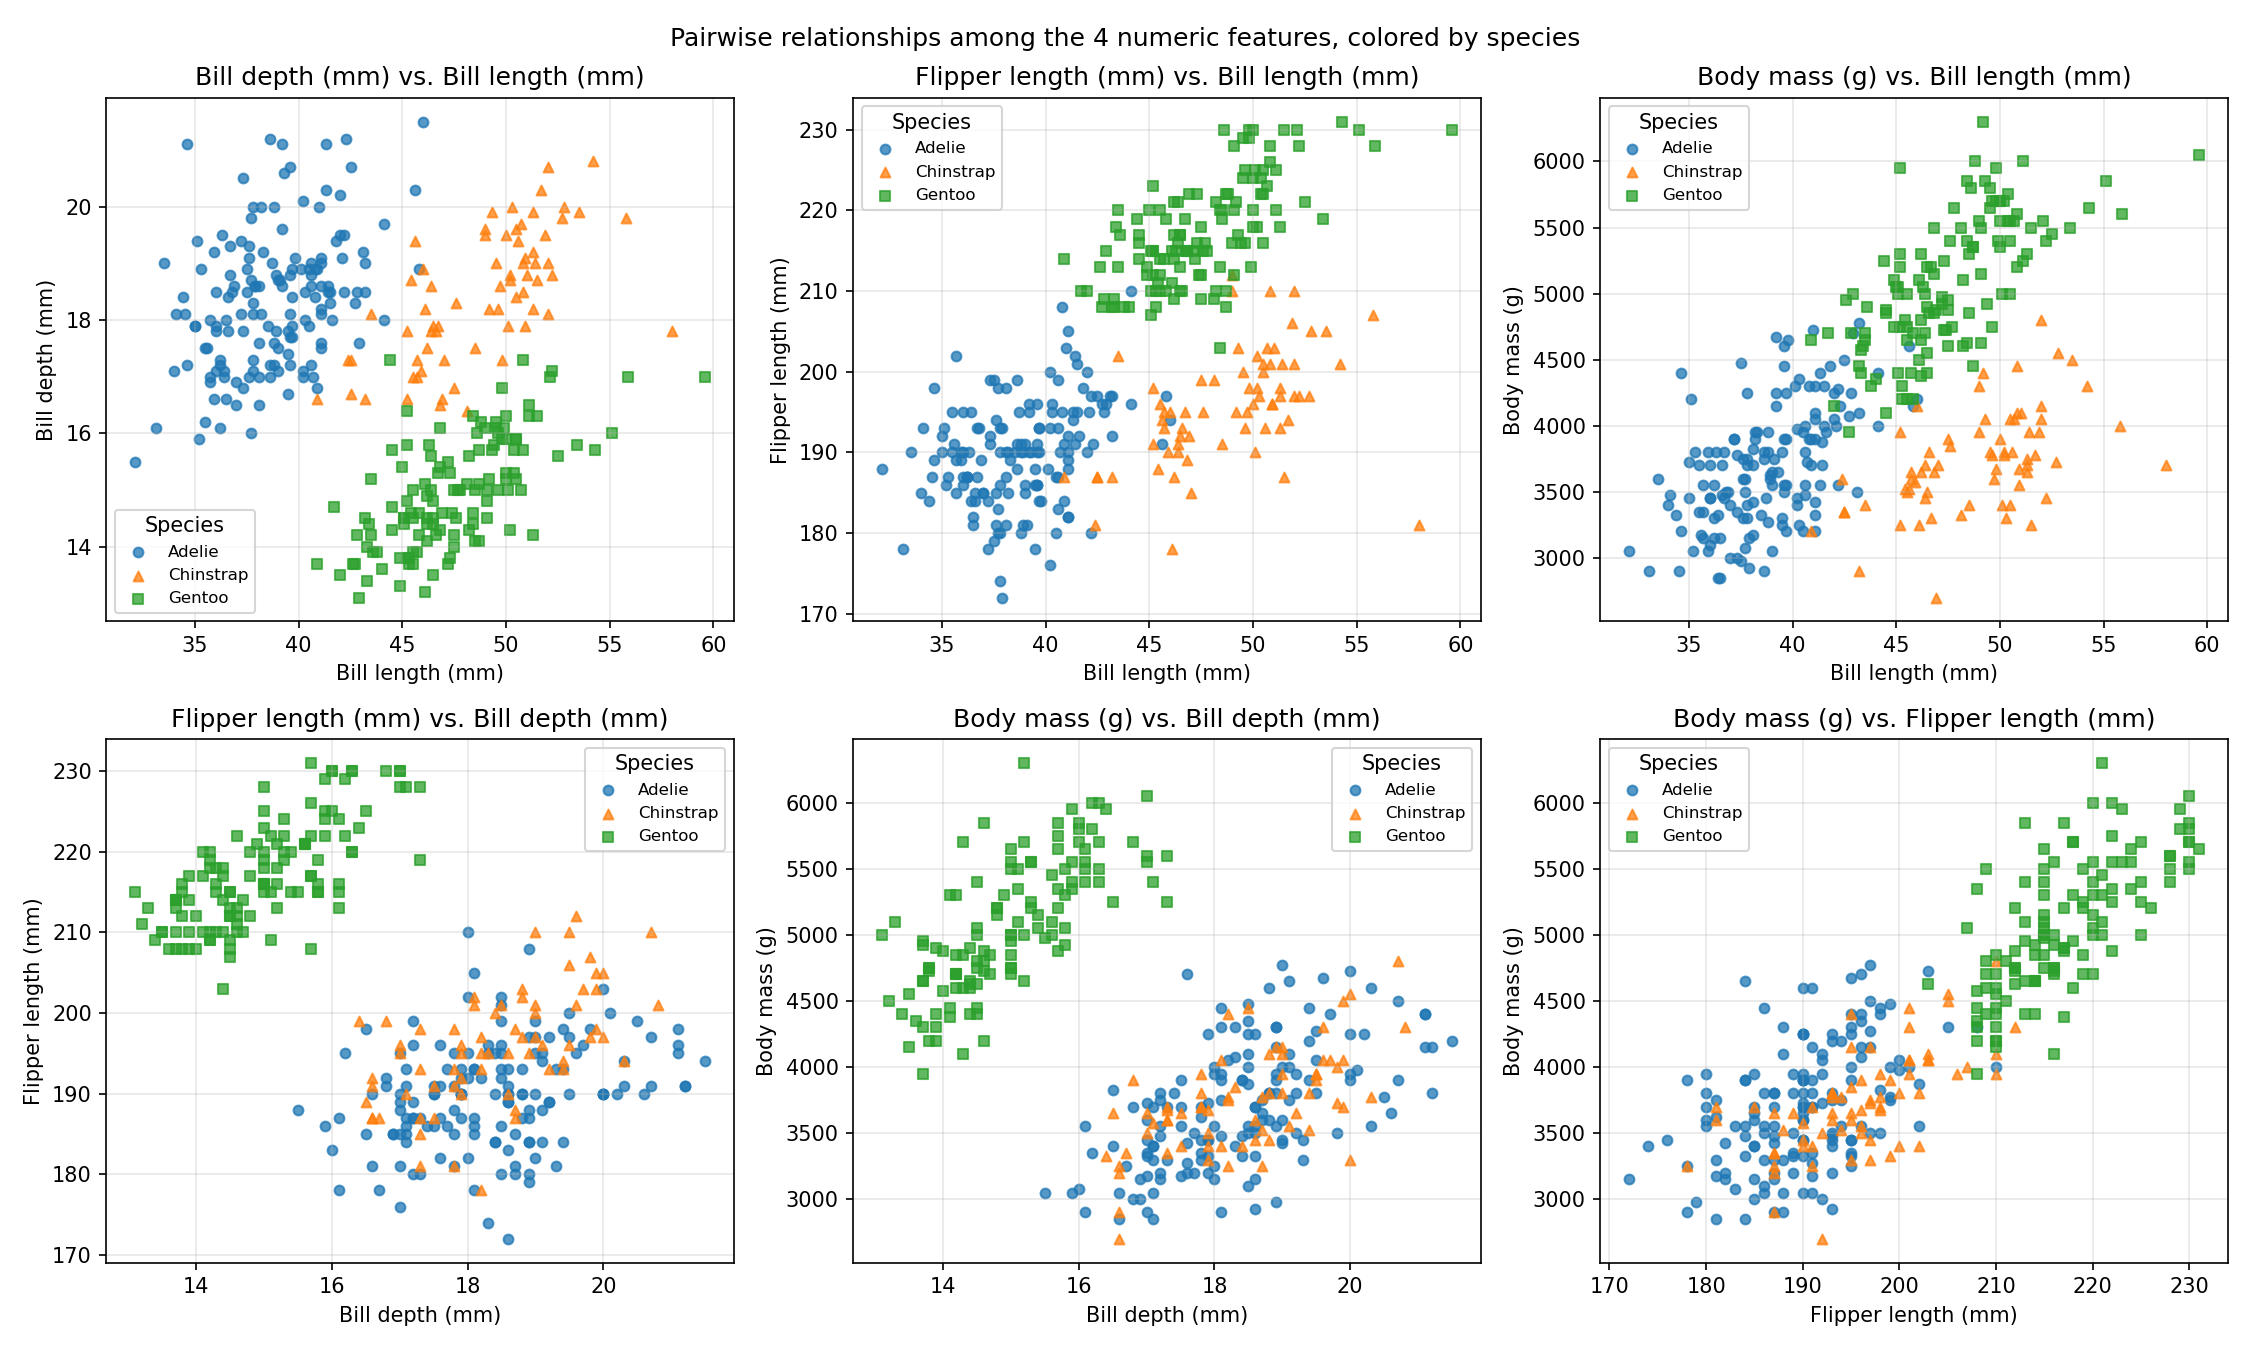
\includegraphics[width=0.95\textwidth]{figures/q5c_scatterplots.png}\end{center}

\paragraph{Pairwise Separation.} Plotting bill depth versus flipper length isolates Gentoo into a distinct cluster (bottom-right region: shallow bill, long flippers). Plotting bill length versus bill depth provides clean separation among all three species simultaneously.

\paragraph{Simpson's Paradox.} Evaluating bill length against bill depth highlights a sign reversal between individual species and the aggregated dataset:
\begin{itemize}\itemsep2pt
\item \textbf{Pooled correlation:} $r = -0.235$
\item \textbf{Within-species correlations:} Adelie $r = +0.391$, Chinstrap $r = +0.654$, Gentoo $r = +0.643$
\end{itemize}
The pooled correlation is negative because Gentoo penguins occupy the long-bill/shallow-depth region of the feature space. Aggregating the distinct species clusters creates an overall downward trend, even though bill length and bill depth are positively correlated within each species.

\newpage
\section*{Q5(d) --- Classification Rules \& Justification}

\paragraph{Decision Rules.}
\begin{Verbatim}
if flipper_length_mm >= 203 and bill_depth_mm < 17.5:
    species = "Gentoo"
elif bill_length_mm >= 43.0:
    species = "Chinstrap"
else:
    species = "Adelie"
\end{Verbatim}

\paragraph{Performance.}
The rules achieve an overall classification accuracy of \textbf{96.49\%} (330 of 342 correct).

\begin{center}\small
\begin{tabular}{lrrr}
\toprule
True $\backslash$ Predicted & Adelie & Chinstrap & Gentoo \\
\midrule
Adelie & \textbf{143} & 8 & 0 \\
Chinstrap & 4 & \textbf{64} & 0 \\
Gentoo & 0 & 0 & \textbf{123} \\
\bottomrule
\end{tabular}
\end{center}

\paragraph{Gentoo Rule Rationale.}
Neither flipper length ($\ge 203$ mm) nor bill depth ($< 17.5$ mm) alone achieves perfect separation, as extreme Adelie samples reach up to 210 mm flipper length and down to 15.5 mm bill depth. However, their conjunction ($\text{flipper} \ge 203\text{ mm} \land \text{depth} < 17.5\text{ mm}$) isolates the Gentoo cluster perfectly with 100\% precision and recall (123/123 Gentoo classified correctly, 0 false positives).

\paragraph{Separating Adelie and Chinstrap.}
Adelie and Chinstrap penguins overlap substantially in bill depth, flipper length, and body mass, leaving bill length as the primary discriminative feature. Adelie's 75th percentile bill length is 40.8 mm, while Chinstrap's 25th percentile is 46.4 mm. A threshold of 43.0 mm sits near the midpoint of this gap. All 12 misclassifications occur within the overlapping bill-length range of 40.9--46.0 mm.

\end{document}
